\chapter{Supplemental for Chapter \refchB}
%\counterwithin{figure}{section}
%\beginsupplement


\begin{figure}[H]
\centering
    % /Users/janet/Dropbox/thesis/tex/chapter2/figures/170314_mapping_fractions--portrait.pdf
    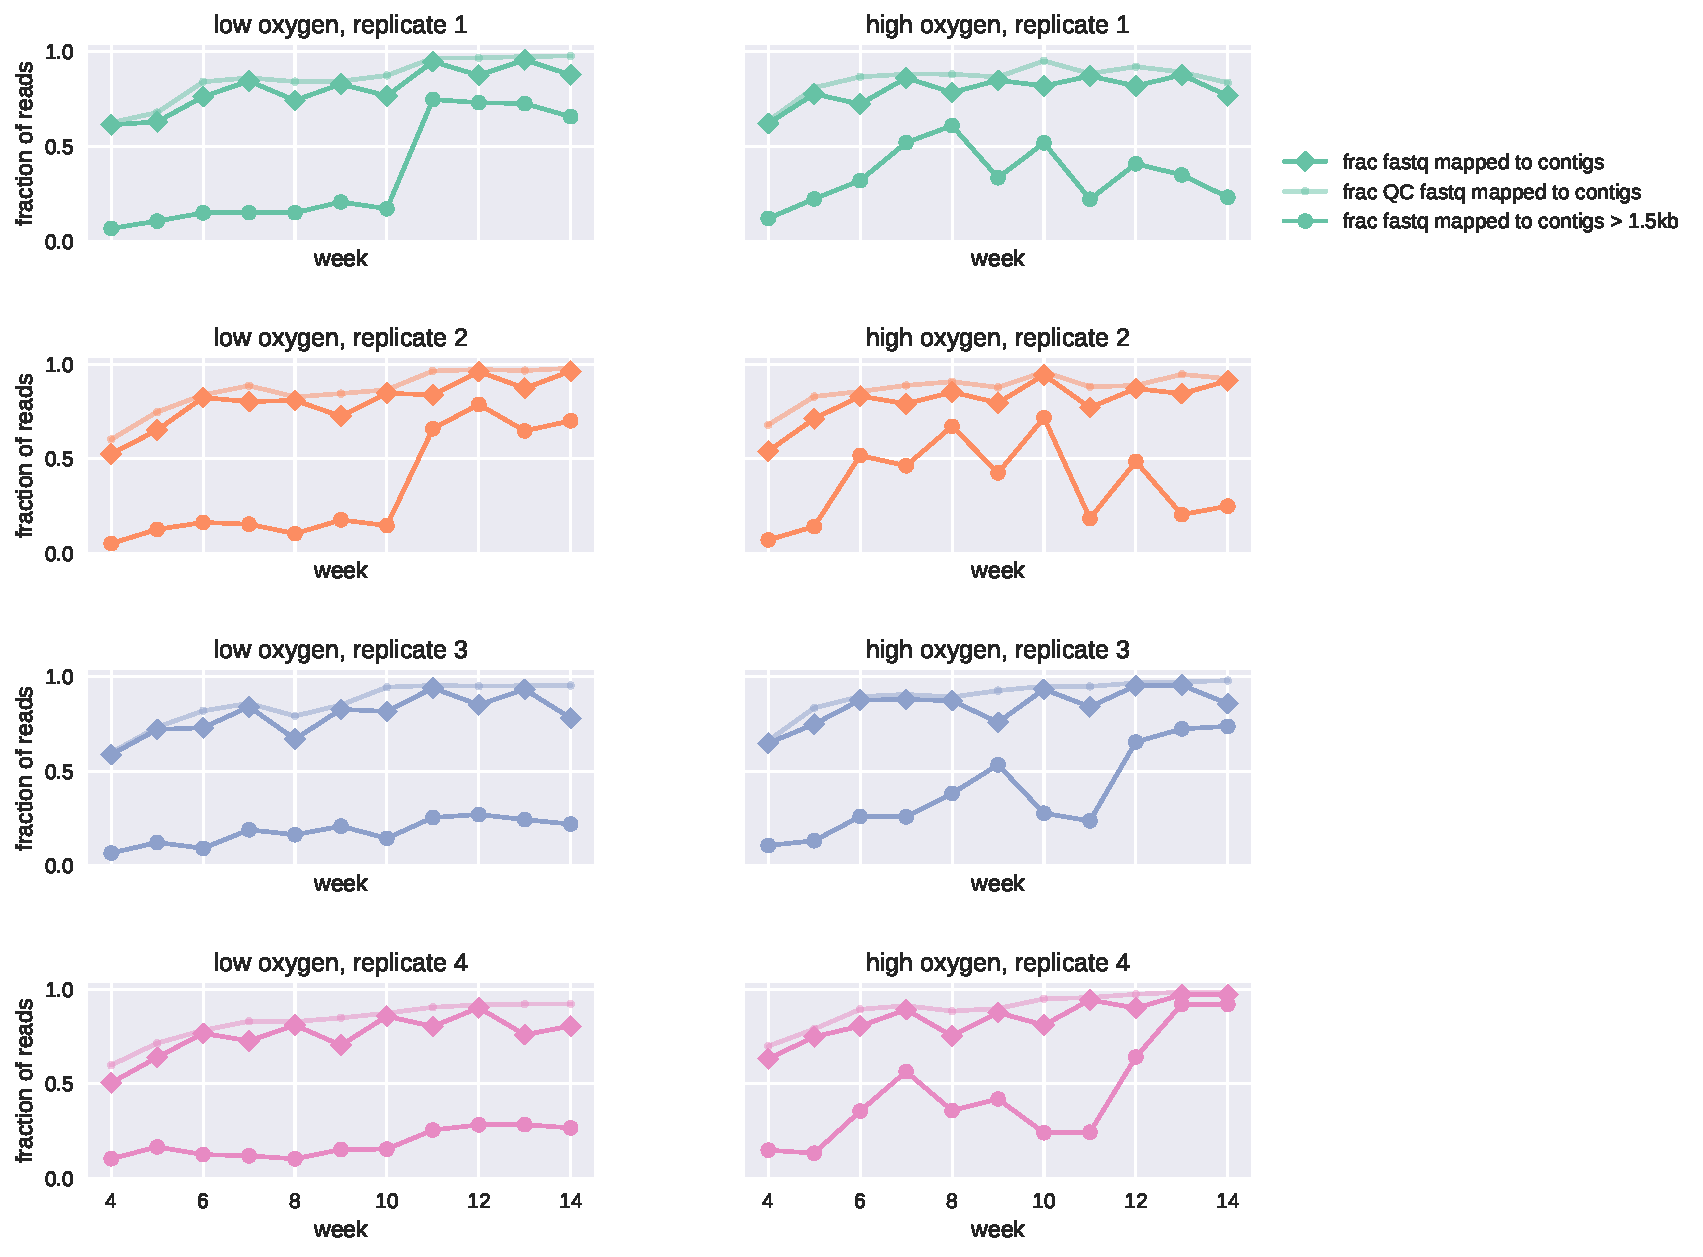
\includegraphics[width=1.0\textwidth]{./tex/chapter2/figures/170314_mapping_fractions--portrait.pdf}
    \begin{singlespace}
    \caption[Fraction of reads mapped to Elviz contigs]{
        Fraction of reads mapped to Elviz contigs.
        The top lines in each sub-plot show the fraction of reads that passed Elviz's QC filter.
        The diamond marks below indicate the fraction of total reads that mapped to contigs.
        The circle marks indicate the fraction that map to contigs with length $>$ 1.5kb, which are most promising for binning.
        }
    \label{fig:frac_elviz_mapped_to_contigs}
    \end{singlespace}
\end{figure}


\begin{figure}[H]
\centering
    % /Users/janet/Dropbox/meta4_bins_data_and_files/170124_current_metabat_analysis_figures/170124_bad_low_o2_samples_have_more_reads_on_short_contigs--binning_not_considered.pdf
    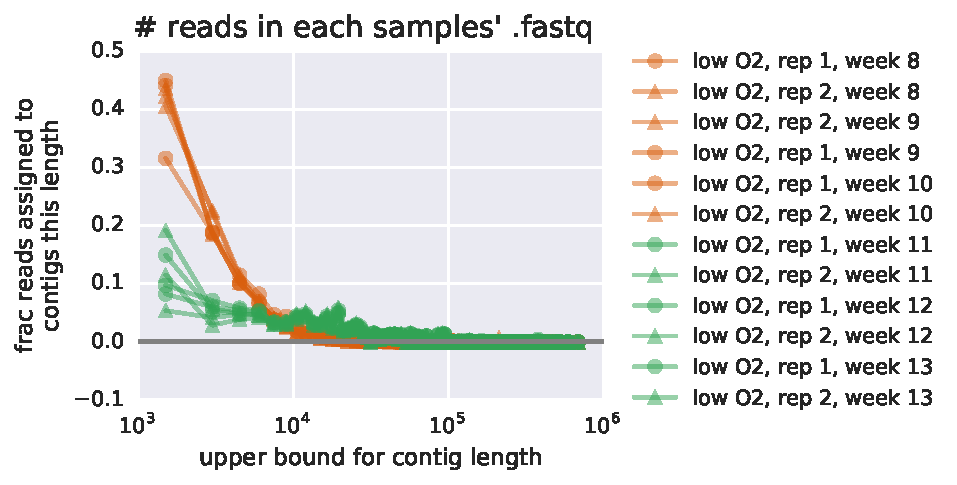
\includegraphics[width=1.0\textwidth]{./tex/chapter2/figures/170124_bad_low_o2_samples_have_more_reads_on_short_contigs--binning_not_considered.pdf}
    \begin{singlespace}
    \caption[Samples best explained by bins have more reads drawn to longer contigs]{
        Samples with metagenomes that are well represented by MetaBAT bins have more reads drawn to longer contigs.}
    \label{fig:contig_dist}
    \end{singlespace}
\end{figure}

\begin{figure}[H]
\centering
    %
    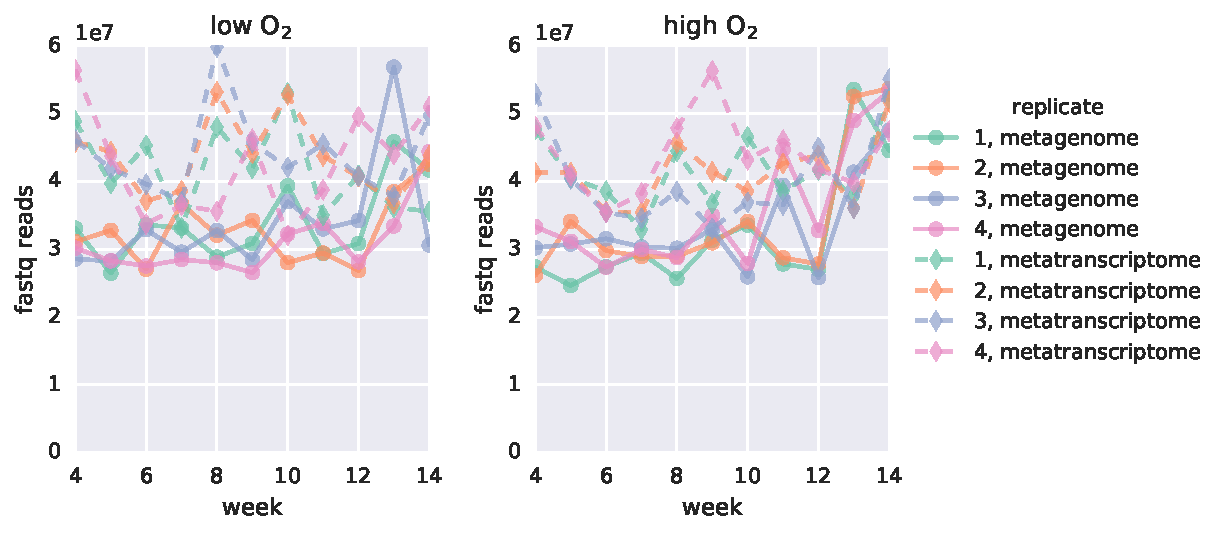
\includegraphics[width=1.0\textwidth]{./tex/chapter2/figures/170326_compare_raw_fastq_reads.pdf}
    \begin{singlespace}
    \caption[Number of reads in metagenomes and metatranscriptomes, by sample]{
        Number of reads in metagenomes and metatranscriptomes, by sample.}
    \label{fig:fastq_reads}
    \end{singlespace}
\end{figure}

